% !TeX spellcheck = hu_HU
% !TeX encoding = UTF-8
% !TeX program = xelatex
%----------------------------------------------------------------------------
\chapter{TPSC scenario-ból automata készítése}
%----------------------------------------------------------------------------

A monitorozás alapja, hogy TPSC scenario-kból időzített automatákat (Timed Automata) tudjunk készíteni. Egy TA állapotokból, elfogadó állapotokból, feltételekből, akciókból és bemenetekkel címkézett állapotátmenetekből áll. Akkor fogad el egy bemenet sorozatot, ha ennek során elérünk az automata végállapotába. Ha elfogadó állapotot érünk el, akkor az a monitor szempontjából hibát jelent. Az alapelv az az, hogy minden TPSC elemhez tartozik egy minta automata (pattern) ami leírja a szemantikáját. Például a 5. és 6. ábrákon láthatóak a különböző PSC üzenetekhez tartozó minták.

\begin{figure}[!ht]
    \centering
    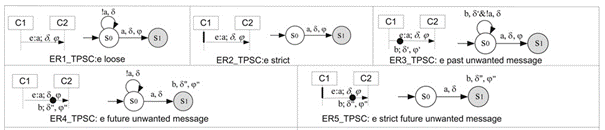
\includegraphics[width=150mm, keepaspectratio]{figures/5abra.png}
    \caption{Sima üzenetekhez tartozó minták[2].}
\end{figure}

\begin{figure}[!ht]
    \centering
    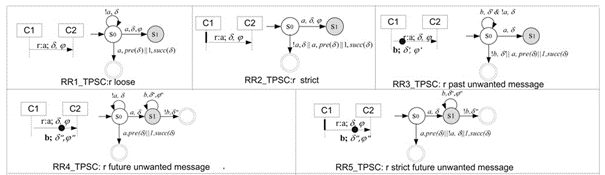
\includegraphics[width=150mm, keepaspectratio]{figures/6abra.png}
    \caption{Elvárt üzenetekhez tartozó minták[2].}
\end{figure}

A minta automatánkban található szürke állapotok reprezentálják a végállapotokat. A megkötéseket az automatáknál egy átmenettel definiáljuk ami a nem kívánt üzenetek negáltjainak az ÉS kapcsolata. Például az 5. ábrán lévő 3. automata mintán látható „b, $\delta ’\&!a, \delta$” címkéjű hurokélen, a „b” azt jelzi, hogy amig nem jött nem kivánt üzenet addig maradjunk az S0 állapotban. A címke teljes jelentése az, hogy ha $\delta$’ időn belül nem jött nem kivánt üzenet és $\delta$ időn belül nem az „a” üzenet jött akkor maradjunk az s0 állapotban. Ezekből az automata részekből lesznek meghatározott illesztési szabályokkal a scenario-hoz tartozó teljes időzített automaták. Ennek az az alapelve, hogy a scenario-n végig menve az előző minta végállapotát a következő minta kezdőállapotával kell egyesíteni. Ezt a folyamatot mutatják be a 7., 8. és 9. ábrák.

\begin{figure}[!ht]
    \centering
    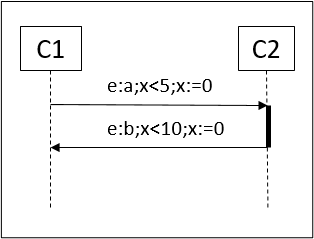
\includegraphics[width=150mm, keepaspectratio]{figures/7abra.png}
    \caption{TPSC részlet.}
\end{figure}

\begin{figure}[!ht]
    \centering
    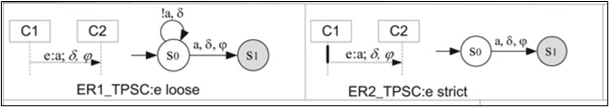
\includegraphics[width=150mm, keepaspectratio]{figures/8abra.png}
    \caption{Alkalmazott automata minták.}
\end{figure}

\begin{figure}[!ht]
    \centering
    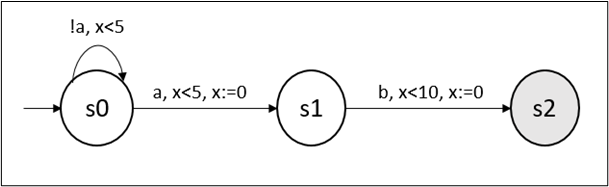
\includegraphics[width=150mm, keepaspectratio]{figures/9abra.png}
    \caption{Az összeállított automata.}
\end{figure}